\large Schreibe ein Python-Script, das einen zufälligen Parcour über das Lavabecken generiert.
\begin{itemize}
	\item Um das Lavabecken und den restlichen Rahmen zu generieren, führe das Initiliasierungsscript im Terminal aus.
	\begin{lstlisting}[language=sh]
python lava_runner_initializer.py
	\end{lstlisting}
	\item Binde die Minecraft-Bibliothek ein, um mit dem Spiel zu kommunizieren.
	\begin{lstlisting}[language=Python]
import mcpi.minecraft as minecraft
	\end{lstlisting}
	
	\item Öffne die Datei \texttt{lava\_runner.py} mit dem Editor. Diese Datei enthält bereits Code und muss lediglich im gekennzeichneten Bereich erweitert werden.
	
	\item Die Variablen \texttt{x}, \texttt{y}, \texttt{z} beschreiben die Position des zu setzenden Steins, \texttt{x\_boundary} und \texttt{z\_boundary} sind die Grenzen der Arena und markieren das Ende des Pfades.
	
	\item Schreibe eine Schleife, die abbricht, sobald die generierte Position über die Grenze \texttt{x\_boundary} oder \texttt{z\_boundary} tritt.

	\item Setze mit \texttt{setBlock(x\_pos, y\_pos, z\_pos, block)}  einen Eisblock (\texttt{block.ICE}) an die zuletzt generierte Position.

	\item Berechne eine zufällige Position, an der der nächste Block platziert werden soll. Nutze dafür die folgende Funktion:
		\begin{lstlisting}[language=Python]
random.randint(lower_bound, upper_bound)
		\end{lstlisting}
	Dabei soll die nächste Position in der y-Achse maximal 1 größer sein als die vorherige Position. Für die x- und z-Achse gilt, dass die nächste Position mindestens 1 und maximal 2 größer sein soll als die vorherige.
		
	\item Frage mit einer \texttt{if}-Bedingung die generierte Position ab und überprüfe, ob diese von Steve erreichbar ist (siehe Abbildung). Kann die neue Position nicht erreicht werden, breche den aktuellen Schleifendurchlauf mit \texttt{continue} ab, falls doch, ersetze die alte Position durch die gerade generierte Position.
\end{itemize}
\begin{figure}
\centering
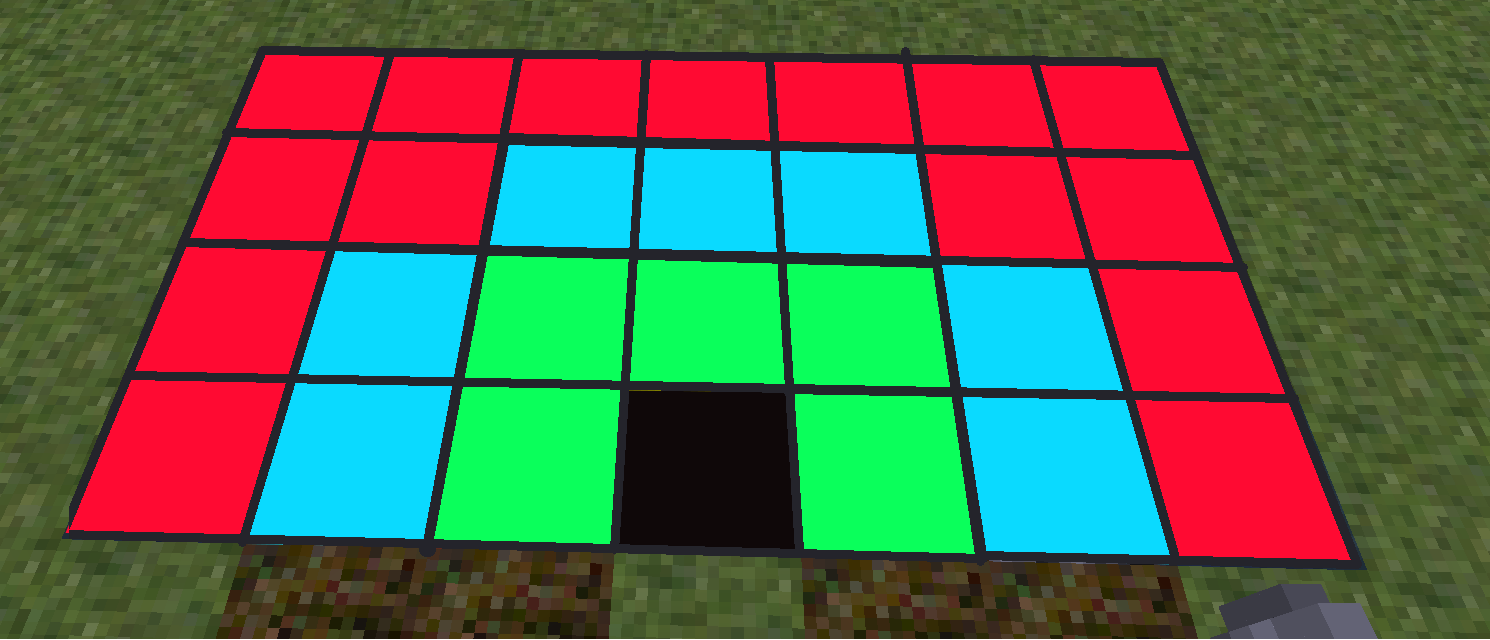
\includegraphics[scale=0.25]{src/lava_runner/res/1layer.png}
\end{figure}
	Das schwarz markierte Feld stellt die Position des vorherigen Blocks dar, die roten Felder sind nicht erreichbar, weshalb ein Block verworfen werden soll, falls er zufällig auf diesem Feld platziert werden soll. Die zu erreichenden Blöcke gilt auch für die Ebene in der sich der Spieler befindet.